
%%%%%%%%%%%%%%%%%%%%%%%%%%%%%%%%%%%%%%%%%%%%%%%%%%%%%%%%%%%%%%%%%%%%%%%%
\chapter{Background}
\label{chap:background}
%%%%%%%%%%%%%%%%%%%%%%%%%%%%%%%%%%%%%%%%%%%%%%%%%%%%%%%%%%%%%%%%%%%%%%%%

This chapter sets the stage for the three typed calculi we are going to present
in later chapters by expanding upon some relevant topics from the introduction.
In \cref{bg:sec:intersection} we start with the traditional formulation of
intersection types, followed by an introduction of the merge operator and the
issue of coherence. We then review the \oname
calculus~\citep{oliveira2016disjoint}, the first calculus featuring disjoint
intersection types, and briefly discuss how disjointness achieves coherence. In
\cref{sec:bg:mixin:trait} we review the concepts of mixins and traits, their
drawbacks and strengths. In \cref{sec:ernst} we introduce family polymorphism by
means of presenting \citeauthor{ernst2004expression}'s elegant
solution~\citep{ernst2004expression} to the expression problem.
\Cref{sec:bg:object} reviews the denotational model of inheritance. Finally in
\cref{sec:bg:lr} we give a simple introduction to program equivalence and
logical relations.




\section{Intersection Types}
\label{bg:sec:intersection}


Intersection types in the pure lambda calculus were developed in the late
1970s by \citet{coppoInter}, and independently by \citet{pottinger1980type}. The
original motivation for intersection types was to devise a
type-assignment system \`a la Curry~\citep{CurryFeys} that satisfies the
following two properties:
\begin{enumerate}
\item The typing of a term should be preserved under $\beta$-conversion. (Under
  Curry's system, $\beta$-reduction preserves types but $\beta$-expansion, in
  general, does not.)
\item Every (strongly) normalizable term has a meaningful type. (We refer the
  reader to their paper for a precise definition of ``meaningful''.)
\end{enumerate}

The idea of intersection types is remarkably simple and natural. From the
set-theoretic perspective, an intersection type $[[A & B]]$ for every pair of
types $[[A]]$ and $[[B]]$ is thought of as containing all the elements of
$[[A]]$ that are also elements of $[[B]]$; from the type-theoretic point of
view, $[[A & B]]$ is a subtype of $[[A]]$, as well as of $[[B]]$; from the
order-theoretic point of view, $[[A & B]]$ is a greatest lower bound of $[[A]]$
and $[[B]]$.\footnote{Note that we say ``a'' rather than ``the'' because
  greatest lower bounds are not unique, but they are all ``equal'' to $[[A & B]]$
  in a sense that will be made precise in \cref{sec:category}.} In the literature of object-oriented programming,
intersection types are long known to model \emph{multiple inheritance}~\citep{compagnoni1996higher}.
The intuition is that if we read the
subtyping $[[A <: B]]$ as ``$[[A]]$ is a subclass of $[[B]]$'', then $[[A & B]]$
is a ``name'' of a class with all the common properties of $[[A]]$ and $[[B]]$. Of
course, this analog is not exact, in the same sense that inheritance is not
subtyping~\citep{cook1989inheritance}. But it is intuitively appealing, and as
we will see, can be made more precise in a sufficiently enriched calculus based
on intersection types. More pragmatically, many programming languages, such as
Scala, TypeScript, Flow and Ceylon adopt some form of intersection types. For example, in Scala
we can express a class \lstinline{A} implements \emph{both} \lstinline{B} and \lstinline{C} by the following declaration:
\begin{lstlisting}[language=Scala]
  class A extends B with C
\end{lstlisting}
where \lstinline[language=Scala]{B with C} denotes an intersection type between
\lstinline{B} and \lstinline{C}.

% What may seem surprising to OO programmers is that $[[A & B]]$ can also be viewed as a natural analog of \emph{multiple inheritance}. If
% we read the subtyping $[[A <: B]]$ as ``$[[A]]$ is a subclass of $[[B]]$'', then
% $[[A & B]]$ is a name of a class with all the common properties of $[[A]]$ and
% $[[B]]$.

\paragraph{Intersection subtyping.}


\newcommand{\rulehl}[1]{}

Three subtyping rules capture the order-theoretic properties of intersection types:
\begin{mathpar}
  \inferrule*[lab=S-interL]{ }{ [[A & B <: A]] } \and
  \inferrule*[lab=S-interR]{ }{ [[A & B <: B]] } \and
  \inferrule*[lab=S-inter]{ [[C <: A]] \\ [[ C <: B  ]]  }{ [[C <: A & B ]] }
\end{mathpar}
Two nice consequences follow:
\begin{enumerate}
\item The top type $[[Top]]$ can be regarded as the 0-ary form of intersection. It is
  a maximum element of the subtyping ordering, i.e., $[[A <: Top]]$ for every
  type $[[A]]$.
\item Multi-field record types can be thought of as an intersection of
  single-field record types. Thus, instead of
  \[
    [[ {  l1 : A1, ... , ln : An   }       ]]
  \]
  we can write
  \[
    [[ { l1 : A1} & ... & {ln : An} ]]
  \]
  Note that the width and depth subtyping of records become a
  consequence of intersection subtyping.
\end{enumerate}


\paragraph{Distributivity rules.}

Two additional subtyping rules are usually found in the literature of
intersection types (e.g., see \citet{reynolds1988preliminary, Barendregt_1983}).
The first one captures the relation between intersections and function spaces,
allowing intersections to distribute over the right-hand side of $[[->]]$'s:
\[
    \drule{S-distArr}
\]
Note that the other direction is also derivable (cf. \cref{sec:typesystem}).
The second rule captures the relation between intersections and (singleton)
records, allowing intersections to distribute over record labels:
\[
    \drule{S-distRcd}
\]
These two rules, though intuitively reasonable, will have a strong effect on both
syntactic and semantic properties of the language. For example, \rref{S-distArr} implies that
$[[ Top <: A -> Top ]]$ for any $[[A]]$; and \rref{S-distRcd} implies that $[[  Top <: {l : Top} ]]$.

\paragraph{Intersection typing.}

The introduction rule of intersection types says that a term $[[ee]]$ can be
given type $[[A & B]]$ if it inhabits both $[[A]]$ and $[[B]]$:
\[
    \drule{interI}
\]
The corresponding elimination rule allows us to derive, given a derivation of
$[[ ee : A1 & A2 ]]$, that $[[ee : A1]]$ and $ [[ee : A2]]$. But this already
follows from intersection subtyping and the subsumption rule; so we need not
to add the elimination rule explicitly to the calculus.


\subsection{The Merge Operator}


Intersection types were first incorporated into a practical programming language
``Forsythe'' by \cite{reynolds1988preliminary, reynolds1997design}, who used
them to encode features such as operator overloading by means of a
``merge'' operator $p_1 ,, p_2$---``a construction for intersecting or
`merging' meanings''~\citep[p. 24]{reynolds1997design}.
(\citeauthor{reynolds1997design} actually used single comma $p_1 , p_2$,
but here we follow \citeauthor{dunfield2014elaborating} by using double commas for consistency.) \citeauthor{reynolds1997design}
demonstrated the power of the merge operator by developing an encoding of
records by using intersection types; similar ideas also appear in
\citet{Castagna_1992}. The idea is to have only single-field records with the introduction form $[[ { l = ee } ]]$ of type $[[ {l : A} ]]$ and
the elimination form $[[ee.l]]$ (record projection). Thus instead of
\[
  [[ {  l1 = ee1, ... , ln = een   }       ]]
\]
we can write
\[
  [[ { l1 = ee1} ,, ... ,, {ln = een} ]]
\]
which plays nicely with the syntactic sugar of multi-field record types as
an intersection of single-field record types.

Recently, \citet{dunfield2014elaborating} developed a method for
elaborating intersections and unions into products and sums. Central to his
system is a source-level \emph{merge operator} $[[ee1 ,, ee2]]$, reminiscent
of Forsythe~\citep{reynolds1997design}, which embodies several computationally
distinct terms, and can be checked against various parts of an intersection
type. In his system, the introduction form of intersection types is still
\rref{interI}, and two additional rules for the merge operator are added:
\begin{mathpar}
  \drule{mergeL}
  \drule{mergeR}
\end{mathpar}
In other words, a merge expression can choose to type one subterm and ignore the
other. In combination of \rref{interI}, they allow to type check
two distinct implementations $[[ee1]]$ and $[[ee2]]$ with completely different
types $[[A1]]$ and $[[A2]]$ of the intersection. For example, let $[[ee1]] = [[\x . x]]$ and $[[ee2]] = 1$,
then the type $[[ (nat -> nat) & nat ]]$ is inhabited by $[[ ee1 ,, ee2  ]]$:
\[
  \inferrule*[right=\rref*{interI}]
  { \inferrule*[right=\rref*{mergeL}]
    { [[ ee1 : nat -> nat  ]] }
    {[[ee1 ,, ee2 : nat -> nat]]}
    \\
    \inferrule*[right=\rref*{mergeR}]
    { [[ ee2 : nat  ]] }
    {[[ee1 ,, ee2 : nat]]}
  }
  { [[  ee1 ,, ee2 : (nat -> nat) & nat   ]] }
\]

\citeauthor{dunfield2014elaborating} showed how to give a semantics to a
calculus with unrestricted intersection types by a type-directed elaboration to
a simply-typed lambda calculus extended with products. For example, the
expression $[[ (\x . x) ,, 1 ]]$ elaborates to a pair $[[ <\x. x , 1> ]]$. As
usual, his system does not have explicit source-level intersection eliminations;
elaboration puts all needed projections into the target program. For instance,
the same expression $[[ (\x . x) ,, 1 ]]$, when checked against $[[nat]]$, elaborates to $[[ pp2 <\x. x , 1> ]]$. The
type-directed elaboration is elegant, type-safe, and serves as the original
foundation for calculi with disjoint intersection types.


\subsection{(In)Coherence}

While \citeauthor{dunfield2014elaborating}'s system is simple and powerful, it
has serious usability issues. More specifically, it lacks the theoretically and
practically important property of \emph{coherence}~\citep{Reynolds_1991}: the
meaning of a target program depends on the choice of elaboration typing
derivation. For example, the expression $[[1 ,, true]]$ has type $[[nat & bool]]$.
It can be used either as an integer or a Boolean, the result is always
clear ($[[1]]$ or $[[true]]$). However, when two types have overlapping
components, it is not at all clear which value to pick. For example, the
expression $[[1 ,, 2]]$ (when checked against $[[nat]]$) could elaborate to
either $1$ or $2$, depending on the particular choice in the implementation.
\citet{dunfield2014elaborating} had a workaround by trying the left part
$[[1]]$ first. It is equally acceptable that one can opt to choose the right part $[[2]]$. But neither is
satisfying from a theoretical point of view.

To recover a coherent semantics, one could limit the merges according to their
surface syntax, as \citeauthor{reynolds1988preliminary} did in Forsythe. But as
\citet{dunfield2014elaborating} pointed out, ``crafting an appropriate syntactic
restriction depends on details of the type system, which is not robust as the
type system is extended''. Another simple idea would be to require all types in
an intersection be \emph{distinct}. This works fine for simple types such as
$[[nat]]$ and $[[bool]]$: $[[nat & bool]]$ is clearly a good intersection. But
it is less clear as to what constituents a ``good'' (read unambiguous) intersection type in
general. A moment of thoughts leads to the following principle: good
intersection types are defined in terms of the subtyping relation. After all, it
is the subtyping relation that defines the behavior of intersection types. A
first attempt would be to require that two types $[[A]]$ and $[[B]]$ can form an
intersection if both types are \emph{not} subtype of each other. At first glance, this
seems to be a reasonable definition because it rules out the problematic merge $[[1 ,, 2]]$. However,
it is still not enough. Consider the following expression (taken from \citet{oliveira2016disjoint}):
\[
[[(1 ,, ss) ,, (2 ,, true)]]
\]
The first component $[[(1 ,, ss)]]$ has type $[[ nat & string ]]$ and the
second component $[[(2 ,, true)]]$ has type $[[ nat & bool ]]$. It is clear that neither of the two is a
subtype of the other. However, extracting an integer from the above expression is
ambiguous ($[[1]]$ or $[[2]]$).

When moving to richer types, it is even less clear how to deal with for example,
intersections of higher-order functions. Consider the following intersection
types (again taken from \citet{oliveira2016disjoint}):
\begin{enumerate}
\item $[[ (nat -> nat) & (string -> string)   ]]$
\item $[[ (string -> nat) & (string -> string)   ]]$
\item $[[ (nat -> string) & (string -> string)   ]]$
\end{enumerate}
We can ask which of those intersection types are qualified as good. It seems
reasonable to expect the first one is good, since both the domain and range
types are different. But the other two are not that obvious to see.
Clearly a formal notion of well-behaved intersection types are called for!

The issue of coherence is addressed in an elegant way by
\citet{oliveira2016disjoint} with the notion of \emph{disjoint intersection types}, as we will discuss next.


\subsection{Disjoint Intersection Types}

\renewcommand{\rulehl}[1]{#1}


\begin{figure}
  \centering
  \drules[Si]{$[[A <: B ~~> e]]$}{Subtyping}{int, top, arr, and, andL, andR}
  \drules[wf]{$[[GG |- A]]$}{Well-formedness of types}{int, top, and, arr}
  \drules[Ti]{$[[GG  |- ee => A ~~> e]]$}{Inference}{top, lit, var, app, anno, merge}
  \drules[Ti]{$[[GG  |- ee <= A ~~> e]]$}{Checking}{abs, sub}
  \caption{Type system of \oname}
  \label{fig:lambdai}
\end{figure}

Disjoint intersection types, first introduced in the \oname
calculus~\citep{oliveira2016disjoint} provide a remedy for the coherence
problem, by imposing restrictions on the uses of merges and on the formation of
intersection types. The syntax of \oname is shown below:
\begin{align*}
  \text{Types} \quad [[A]] &\Coloneqq [[nat]] \mid [[A1 -> A2]] \mid [[A1 & A2]]  \\
  \text{Terms} \quad [[ee]] &\Coloneqq [[ii]] \mid [[x]] \mid [[\x . ee]] \mid [[ee1 ee2]] \mid [[ee1 ,, ee2]] \mid [[ee : A]]
\end{align*}
Its full (bidirectional) type system is shown in \cref{fig:lambdai}. Central
to their system is the notion of \emph{disjointness}. As a first
approximation, for two types $[[A]]$ and $[[B]]$ to be disjoint (written $[[A ** B]]$),
they must not have any sub-components sharing the same type. In a type
system without $[[Top]]$, this can be ensured by the following specification:

\begin{definition}[Simple disjointness] \label{def:disjoint_spec}
  $[[A ** B]] \defeq  \nexists C.\ [[A <: C]] \land [[B <: C]]$
\end{definition}

The disjointness judgment appears in the well-formedness of intersection types
(\rref{wf-and}) and the typing rule of merges (\rref{Ti-merge}).
\Rref{wf-and}---the well-formedness of intersections---enforces that only
disjoint types can form an intersection type: so $[[nat & bool]]$ is
well-formed but $[[nat & nat]]$ is not. \Rref{Ti-merge}---the typing rule for
merges---prevents problematic merges such as $[[1 ,, 2]]$ (because $[[nat]]$ and
$[[nat]]$ are not disjoint), while accepting unambiguous merges such as $[[1 ,, true]]$.
\begin{remark}
  Note that the introduction form for disjoint intersection types
  (\rref{Ti-merge}) is not as expressive as \rref{interI}. For instance, \rref{interI} entails
  the following derivation:
  \[
    \inferrule*{ [[  \x .x : nat -> nat  ]] \\ [[ \x . x : char -> char   ]]    }{  [[\x . x : (nat -> nat) & (char -> char)]]  }
  \]
  which is impossible to express in \oname.
\end{remark}

To ensure that subtyping produces unique coercions, they also employ the notion
of \emph{ordinary types}~\citep{Davies_2000}---those that are not intersection
types---and use the judgment ``$[[ A ord ]]$'' in \rref{Si-andL,Si-andR}.
Ordinary types and disjointness are sufficient to ensure a coherent semantics of
a type system without $[[Top]]$.

$[[Top]]$ brings extra complications, because \cref{def:disjoint_spec} does not
hold anymore ($[[Top]]$ is trivially a supertype of every type). To address this
problem, the notion of \emph{top-like types} was introduced, which are those
types that behave like $[[Top]]$ (such as $[[Top & Top]], [[Top & Top & Top]],
\dots$), and captured by a predicate $ \rceil \cdot \lceil $. An important
observation is that any coercions for top-like types are unique, \emph{even if
  multiple derivations exist}. The meta-function $\llbracket \cdot \rrbracket $
used in \rref{Si-andL,Si-andR} defines coercions for top-like types.
With top-like types,
\cref{def:disjoint_spec} is refined to account for $[[Top]]$, as shown in
\cref{def:disjoint_spec2}.

\begin{definition}[$[[Top]]$-Disjointness] \label{def:disjoint_spec2}
  $[[A ** B]] \defeq \neg \rceil [[A]] \lceil \ \land \ \neg \rceil [[B]] \lceil \ \land \
  (\forall C.\ [[A <: C]] \land [[B <: C]] \Longrightarrow \rceil [[C]] \lceil)$
\end{definition}

However, a careful analysis of \cref{def:disjoint_spec2} shows that intersection
types such as $[[ Top & Top ]]$ and $[[Top & nat]]$ are not well-formed because
their constituent types are not disjoint. This is one of the limitations in
\oname, since ``a merge of two $[[Top]]$-types will always return the same value
regardless of which component of the merge is chosen''~\citep{alpuimdisjoint}.
In other words, $[[Top]]$ is always disjoint to every other type. This
restriction was later lifted in the \fname calculus of \citet{alpuimdisjoint} by
a set of inference rules, but whether a corresponding specification of
disjointness exists or not was not known at that time. We will present a
suitable specification in \cref{sec:category}.


Combined with bidirectional type-checking, \citet{oliveira2016disjoint}
formalized the \oname calculus in Coq and prove that there is at most one
elaboration derivation for any expression, and as a consequence, there is only
one possible target program and thus coherence follows trivially. We refer the
reader to their paper for a detailed account of \oname.

\subsection{Disjoint Polymorphism}
\label{bg:sec:disjoint_poly}


Disjoint polymorphism, first proposed by \citet{alpuimdisjoint} in the \fname
calculus, is a more advanced mechanism to combine disjoint intersection
types with parametric polymorphism. The combination allows objects with
statically unknown types to be composed without conflicts. To understand the
usefulness of disjointness polymorphism, consider the following program (adapted
from \citet{alpuimdisjoint}):
\begin{lstlisting}
mergeBad X (x : X) : X & Int = x ,, 2;
\end{lstlisting}
\lstinline{mergeBad} takes an argument \lstinline{x} of type \lstinline{X} (which is itself a type variable), and merges it with \lstinline{2}.
However, if we were to allow such definition, we could easily create an example where incoherence occurs again:
\begin{lstlisting}
(mergeBad Int 1) : Int -- 1 or 2
\end{lstlisting}
This is essentially the same problem of allowing $[[1 ,, 2]]$, which as we
discussed will cause ambiguity. For \oname, we
know the concrete type for each variable and thus disjointness checking can help
avoid this problematic expression. However, with parametric polymorphism, a
variable could have any types,
including those that are already in the intersection. So a question to ask is to
decide under what conditions a type variable is disjoint with, say,
\lstinline{Int}. This is where \emph{disjointness constraints} come into stage. The key
idea is that since we do not know \emph{a priori} what is the type with which
a type variable can be instantiated, we can restrict the set of types it can be
instantiated to. Let us rewrite the above program as follows:
\begin{lstlisting}
mergeGood [X * Int] (x : X) : X & Int = x ,, 2;
\end{lstlisting}
The only change is the notation \lstinline{[X * Int]}, where the left-side of
\lstinline{*} denotes the type variable being declared, and the right-side
denotes the disjointness constraint(s). Here the disjointness constraint
(\lstinline{Int}) effectively states that the type variable \lstinline{X} can be
instantiated to any types disjoint with \lstinline{Int}. For instance, the expression \lstinline{mergeGood Bool True}
type checks but the expression \lstinline{mergeGood Int 1}
is rejected because \lstinline{Int} (the type argument) is not disjoint with
\lstinline{Int} (the disjointness constraint). Moreover, we can express multiple
constraints using intersection types, for example,
\begin{lstlisting}
mergeThree [X * Int & Bool] (x : X) : X & Int & Bool = x ,, 2 ,, True;
\end{lstlisting}
Here the type variable \lstinline{X} can only be instantiated to types disjoint with both
\lstinline{Int} and \lstinline{Bool}.


In essence disjoint intersection types and disjoint polymorphism retain most of the expressive power of
the merge operator. For example, as noted by \citet{alpuimdisjoint}, they can be
used to model powerful forms of extensible records. However, forcing every
intersection types to be disjoint is unnecessarily restrictive. For instance,
$[[1 : nat & nat]]$ is undoubtedly unambiguous, but is rejected by \oname and
\fname. Another issue is that because of the restriction, \fname lacks a general
substitution lemma; only a restricted form applies, which greatly complicates
the metatheory. Our starting point in this thesis is to lift this restriction
and makes room for more expressiveness for calculi with disjoint intersection
types.

\section{Mixins and Traits}
\label{sec:bg:mixin:trait}


Programmers have long realized that single inheritance is not flexible enough
when it comes to structuring a class hierarchy. For example, consider two
classes in different branches of the inheritance hierarchy, and assume that they
share features not inherited from their (unique) common parent. Attempting to
share the implementation of the common features may lead to putting the common
methods \emph{too high} in the hierarchy (i.e., they are forced into their
common parent), and these methods will be inherited by other classes in the same
hierarchy, which may not be desirable. On the other hand, putting those methods
in a \emph{lower} position results in code duplication. To overcome this
limitation, \emph{multiple inheritance} was proposed as a generalization of
single inheritance. However, as \citet{cook:multi} put it:
\begin{quote}
  ``Multiple inheritance is good, but there is no good way to do it.''
\end{quote}
One of the problems in multiple inheritance is the ambiguity issue that arises
when conflicting features are inherited along different paths. A classic
situation is the \emph{diamond problem}~\citep{bracha1990mixin} where a class
inherits from two parent classes that have a common superclass, as depicted by
\cref{fig:diamond}.


\begin{figure}
  \centering
  \begin{subfigure}[b]{0.45\textwidth}
    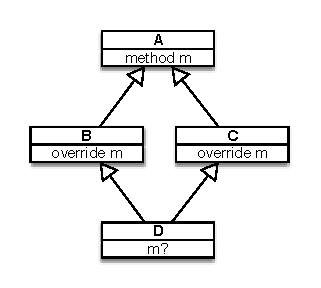
\includegraphics{figures/diamond.eps}
    \subcaption{The diamond problem} \label{fig:diamond}
  \end{subfigure} ~
  \begin{subfigure}[b]{0.45\textwidth}
    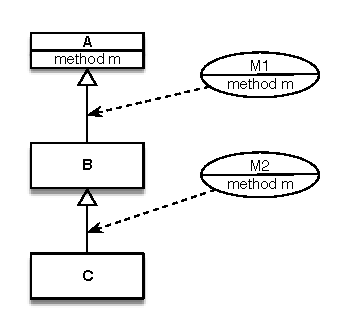
\includegraphics{figures/mixin.eps}
    \subcaption{Mixin composition} \label{fig:mixin}
  \end{subfigure}
  \caption{Multiple inheritance and mixins}
\end{figure}


Mixins and traits are two well-studied mechanisms to provide some form of
multiple inheritance. Mixins~\citep{bracha1990mixin} provide a simple mechanism
for multiple inheritance without the ambiguity issue. A mixin is a subclass
declaration parameterized over a superclass. Or simply put, a mixin can be
treated as a function from classes to classes. Thus the same mixin can be used to
extend a variety of parent classes with the same set of features.
\Cref{fig:mixin} shows a typical class hierarchy when using mixins. In the mixin
model, a class can inherit from another class by means of single inheritance as
usual. Apart from that, it can also have several mixins applied \emph{one at a time}.
Let us take a close look at \cref{fig:mixin}. Both mixins
\lstinline{M1} and \lstinline{M2} contain a method \lstinline{m}, a question
arises as to which one is inherited in the class \lstinline{C}. The answer is
\lstinline{m} from the mixin \lstinline{M2}. This is because mixin composition
is \emph{linear}: methods defined in mixins appearing later override all the
identically named methods of earlier mixins. While this simple mechanism does
avoid conflicts, it also lead to other problems. For example, though we can
obtain the method \lstinline{m} from the mixin \lstinline{M1} by switching the
order of \lstinline{M1} and \lstinline{M2}, no suitable order of composition
exists to obtain \lstinline{m} from the superclass \lstinline{A}.

In response to the problems in the then compositional models,
\citet{scharli2003traits} proposed a mechanism called \emph{traits} as a
better way to foster code reuse in object-oriented programs. A trait is
essentially \emph{a set of pure methods}, divorced from any class hierarchy. A
trait \emph{provides} a set of methods to implement the behavior, and it may
also specify a set of \emph{required methods} that parameterize the provided
behavior. \Cref{fig:trait} shows a simple trait \lstinline{TCircle}, which
provides two methods \lstinline{hash} and \lstinline{area}, and requires a
method \lstinline{radius}. A class is then constructed by inheriting from a
superclass and incorporating a collection of traits, as shown in
\cref{fig:trait:conflict}. Notice that there is a conflicting method
\lstinline{hash} that is provided by both \lstinline{TCircle} and
\lstinline{TDraw}. This is where the trait model is very different from the
mixin model. Unlike mixins that force a linear order in their composition,
traits can be composed in arbitrary order, and as a consequence, conflicting
methods must be resolved \emph{explicitly}, either by overriding the
conflicting methods, or by excluding a method from all but one trait.
\citet{scharli2003traits} discuss several other issues with mixins, which can be
improved by traits. We refer to their paper for a detailed account of traits.


\begin{figure}
  \centering
  \begin{subfigure}[b]{0.45\textwidth}
    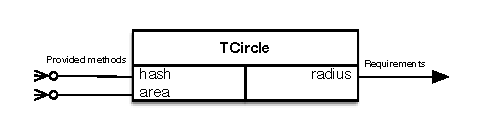
\includegraphics[scale=0.85]{figures/trait1.eps}
    \subcaption{A simple trait} \label{fig:trait}
  \end{subfigure} ~
  \begin{subfigure}[b]{0.45\textwidth}
    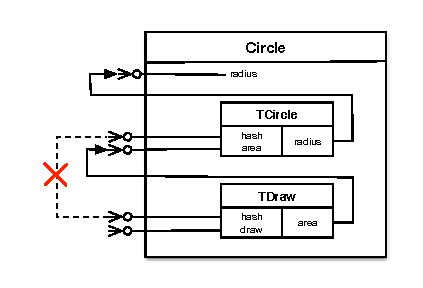
\includegraphics{figures/trait3.eps}
    \subcaption{Trait composition with conflicts} \label{fig:trait:conflict}
  \end{subfigure}
  \caption{Traits and conflicts}
\end{figure}


\section{Family Polymorphism and Nested Composition}
\label{sec:ernst}
% %-------------------------------------------------------------------------------
% \subsection{Motivation: Family Polymorphism}

Family polymorphism~\citep{Ernst_2001} is the ability to simultaneously refine a family of
related classes through inheritance. This is motivated by a need to not only
refine individual classes, but also to preserve and refine their mutual
relationships. \citet{Nystrom_2004} call this \emph{scalable extensibility}:
``the ability to extend a body of code while writing new code proportional to
the differences in functionality''.
%
A well-studied mechanism to achieve family inheritance is \emph{nested
inheritance}~\citep{Nystrom_2004}. Nested inheritance combines two aspects.
Firstly, a class can have nested class members; the outer class is then a
family of (inner) classes. Secondly, when one family extends another, it
inherits (and can override) all the class members, as well as the relationships
within the family between the class members. However,
the members of the new family do not become subtypes of those in the parent family.

\paragraph{The expression problem.}

\citet{ernst2004expression} illustrates the benefits of nested inheritance for modularity
and extensibility with one of the most elegant and concise solutions to the
\emph{expression problem}~\citep{wadler1998expression}. The expression problem,
as surveyed by \citet{togersen:2004}, is to answer the question:
\begin{quote}
  ``To which degree can your application be structured in such a way that both
  the data model and the set of virtual operations over it can be extended
  without the need to modify existing code, without the need for code repetition
  and without run-time type errors.''
\end{quote}
The expression problem is concerned with two-dimensional extensions:
\begin{inparaenum}[(1)]
\item adding new variants to the datatype;
\item and adding new operations on the datatype.
\end{inparaenum}
Depending on the programming style used in the code, it is usually
straightforward to add either new variants or new operations. For example, in an
object-oriented language such as Java where an abstract datatype is represented by means of
classes whose methods are the operations on the datatype, it is easy to extend
the set of variants by writing another class. On the other hand, in a functional
language such as Haskell where the abstract datatype is modeled by means of
algebraic datatypes with a set of pattern matching functions as the operations,
then it is easy to add new operations by writing new pattern matching functions.
In either case, it is much harder to perform both extensions in the
\emph{same} language.


\paragraph{The expression problem, Scandinavian style.}

Nowadays we know many solutions to the expression problem (for example, see
\citet{oliveira2012extensibility, wang2016expression, oliveira09modular,
  swierstra_2008, Zenger-Odersky2005}, to cite a few). Among all of them,
\citeauthor{ernst2004expression}'s solution is perhaps one of the most elegant
solutions out there. \citeauthor{ernst2004expression} solves the expression
problem in the \textsf{gbeta} language~\citep{ernst2000gbeta}, which he adorns with a Java-like syntax for
presentation purposes, for a small abstract syntax tree (AST) example. His
starting point is the code shown in \cref{fig:lang}. The outer class
\lstinline{Lang} contains a family of related AST classes: the common superclass
\lstinline{Exp} and two cases, \lstinline{Lit} for literals and \lstinline{Add}
for addition. The AST comes equipped with one operation, \lstinline{toString},
which is implemented by both cases. Notice that all the inner classes are
\emph{virtual}, in the same sense of virtual methods, which means that they
may be redefined in subclasses of the enclosing class.


\begin{figure}[t]
    \centering
    \begin{subfigure}[b]{0.45\textwidth}
\begin{lstlisting}[language=gbeta]
class Lang {
  virtual class Exp {
    String toString() {}
  }
  virtual class Lit extends Exp {
    int value;
    Lit(int value) {
      this.value = value;
    }
    String toString() {
      return value;
    }
  }
  virtual class Add extends Exp {
    Exp left,right;
    Add(Exp left, Exp right) {
      this.left = left;
      this.right = right;
    }
    String toString() {
      return left + "+" + right;
    }
  }
}
\end{lstlisting}
\subcaption{Base family: the language \lstinline{Lang}} \label{fig:lang}
    \end{subfigure} ~
    \begin{subfigure}[b]{0.5\textwidth}
\begin{lstlisting}[language=gbeta,  xleftmargin=1mm]
// Adding a new operation
class LangEval extends Lang {
  refine class Exp {
    int eval() {}
  }
  refine class Lit {
    int eval { return value; }
  }
  refine class Add {
    int eval { return
      left.eval() + right.eval();
    }
  }
}
// Adding a new case
class LangNeg extends Lang {
  virtual class Neg extends Exp {
    Neg(Exp exp) { this.exp = exp; }
    String toString() {
      return "-(" + exp + ")";
    }
    Exp exp;
  }
}
\end{lstlisting}
\subcaption{Extending in two dimensions} \label{fig:extend}
    \end{subfigure}
    \caption{The expression problem, Scandinavian Style}
\end{figure}

\paragraph{Adding a new operation.}

One way to extend the family is to add an additional evaluation operation, as
shown in the top half of \cref{fig:extend}. This is done by subclassing the
\lstinline{Lang} class and refining all the contained classes by implementing
the additional \lstinline{eval} method. The semantics of the keyword
\lstinline[language=gbeta]{refine} is that the virtual class is constrained to
be a subclass of the new declaration. In other words, \lstinline{Exp},
\lstinline{Lit} and \lstinline{Add} are all extended with the \lstinline{eval}
method. Note that the inheritance between, e.g., \lstinline{Lang.Exp} and
\lstinline{Lang.Lit} is transferred to \lstinline{LangEval.Exp} and
\lstinline{LangEval.Lit}. Similarly, the \lstinline{Lang.Exp} type of the
\lstinline{left} and \lstinline{right} fields in \lstinline{Lang.Add} is
automatically refined to \lstinline{LangEval.Exp} in \lstinline{LangEval.Add}.

\paragraph{Adding a new case.}

A second dimension to extend the family is to add a case for negation, shown in
the bottom half of \cref{fig:extend}. This is similarly achieved by subclassing
\lstinline{Lang}, and now adding a new contained virtual class \lstinline{Neg}
that represents the unary negation operator. Note that \lstinline{Neg} is
declared to be a subclass of \lstinline{Exp}, which means that the extension to
\lstinline{Exp} will also be added to \lstinline{Neg}.


\paragraph{Combining both extensions.}

Finally, the two extensions are naturally combined by means of multiple
inheritance, closing the diamond. (\citeauthor{ernst2004expression} uses the
symbol $\oplus$ to play the role of ``intersecting'' two classes.)
\begin{lstlisting}[language=gbeta]
class LangNegEval extends LangEval o+o LangNeg {
  refine class Neg {
    int eval() { return -exp.eval(); }
  }
}
\end{lstlisting}
The only effort required is to implement the one missing operation
case, evaluation of negated expressions.




\section{Functional Object Encodings}

\label{sec:bg:object}

\citet{cook1989denotational} developed a method for modeling inheritance in the
presence of self-reference, based on the fixed-point semantics of recursive
definitions. In their model, the interpretation of inheritance is taken as a
mechanism of \emph{incremental programming}, where new programs are developed
by specifying the \emph{modification}---i.e., how they differ from existing
ones; self-reference in the original definition must be changed to refer to the
modified definition.

We use an example to illustrate the encodings of classes and objects. First we
define a class of points. Points have two components \lstinline{x} and
\lstinline{y} to specify their locations. The \lstinline{dist} method computes
their (Euclidean) distance from the origin. The following is a Scala class
\lstinline{Point}:
\begin{lstlisting}[language=Scala]
class Point(x : Int, y : Int) {
  def dist() = sqrt(square(this.x) + square(this.y))
}
\end{lstlisting}

In a purely functional setting, objects are modeled as records whose fields
represent methods. The class \lstinline{Point} is then modeled as a
\emph{generator} \lstinline{PointGen(a, b)}, defined as follows:
\begin{lstlisting}[language=simple]
PointGen(a, b) = lamthis.
  { x = a
  , y = b
  , dist() = sqrt(square(this.x) + square(this.y))
  }
\end{lstlisting}
Notice that the keyword \lstinline{this} is modeled as a formal parameter of the
function. % When applied to the coordinates of a new point, \lstinline{PointGen}
% returns a generator whose fixed point is a point object.
Formally speaking, a function intended to specify a fixed point whose formal
parameter represents self-reference is called a generator.

A point $(3, 4)$ is created by taking a fixed point of \lstinline{PointGen(3, 4)} using a
\emph{lazy recursive} let binding:
\begin{lstlisting}[language=simple]
p = letrec this = PointGen(3, 4, this) in this
\end{lstlisting}
and method invocation on objects is simply record projections:
\lstinline{p.dist()} evaluates to $5$ as expected.

\paragraph{Modeling inheritance.}

Inheritance allows a new class to be defined by adding or replacing methods in
an existing class. We illustrate this by defining another class \lstinline{Circle}:
\begin{lstlisting}[language=Scala]
class Circle(x : Int, y : Int, radius : Int) extends Point(x, y) {
  override def dist() = abs(super.dist() - this.radius)
}
\end{lstlisting}
The class \lstinline{Circle} inherits from \lstinline{Point} and redefines the
method \lstinline{dist} to mean the closest distance from the circle to the
origin. It reuses the original \lstinline{dist} method in the body.
To correctly model inheritance, there are three aspects to note:
\begin{inparaenum}[(1)]
\item the addition or replacement of methods,
\item the redirection of \lstinline{this} in the original generator to the modified methods,
\item and the binding of \lstinline{super} to refer to the original methods.
\end{inparaenum}

Inheritance is modeled as a function that takes a generator and returns a new
generator. Such functions are called \emph{wrappers}. Below we give a wrapper
for the subclass \lstinline{Circle}:
\begin{lstlisting}[language=simple]
CircleWrapper(a, b, r) = lamthis. lamsuper.
  { radius = r
  , dist() = abs(super.dist() - this.radius)
  }
\end{lstlisting}
\lstinline{CircleWrapper(a, b, r)} is defined as a function of two arguments,
one representing \lstinline{this} and the other representing \lstinline{super}.

The generator for the class \lstinline{Circle} can now be defined by
applying \lstinline{CircleWrapper} to \lstinline{PointGen} as follows:
\begin{lstlisting}[language=simple]
CircleGen(a, b, r) = lamthis.
  let super = PointGen(a, b, this)
  in (CircleWrapper(a, b, r, this) super) o+o super
\end{lstlisting}
That is, a wrapper works by first distributing \lstinline{this} to both the
wrapper and the original generator. Then the modification is applied to the
original record definition to produce a modification record. Note that at this
stage, the binding of \lstinline{this} correctly refers to the modification,
while the binding of \lstinline{super} refers to the original record. Finally
the modification record is combined with the original record using $\oplus$.
(\lstinline{M o+o N} is defined in a way such that any method defined in \lstinline{M}
replaces the corresponding method defined in \lstinline{N}.)


\section{Program Equivalence and Logical Relations}

\label{sec:bg:lr}


Proving equivalence of programs is important for a variety of settings, e.g.,
verifying the correctness of compiler optimization and other program
transformations, establishing the property that program behavior is independent
of the representation of an abstract type. The latter---so-called the property of
\emph{representation independence}---is particularly relevant for programmers
and clients in the sense that a client will not be able to tell a difference if
one implementation is swapped by another, as long as they all adhere to the same
interface.

Program equivalence is generally defined in terms of \emph{contextual
  equivalence}. The intuition is that two programs are equivalent if we
\emph{cannot} tell them apart in any context. More formally, we introduce the
notion of \emph{expression contexts}. An expression context $[[cc]]$ is a term
with a single hole $[[__]]$ (possibly under some binders) in it. Take the
simply-typed lambda calculus (STLC) for example, the syntax of expression contexts is as
follows:
\[
\text{Contexts} \quad [[cc]] \Coloneqq [[__]] \mid [[\x . cc]] \mid [[cc e]] \mid [[e cc]]
\]
The only operation of expression contexts is \emph{replacement}, which is the
process of filling a hole in an expression context $[[cc]]$ with an expression
$[[e]]$, written $[[ cc{e} ]]$. An important point is that replacement
\emph{is not} substitution, that is, the free variables of $[[e]]$ that are
exposed by $[[cc]]$ are captured by replacement. The static semantics of STLC
is extended to expression contexts by defining the typing judgment
\[
  [[cc : (gg |- T) ~> (gg' |- T')]]
\]
where $([[gg |- T]])$ indicates the type of the hole. This judgment is
inductively defined so that if $[[gg |- e : T]]$, then $[[gg' |- cc{e} : T']]$.

\paragraph{Contextual equivalence.}

We define a \emph{complete program} to mean any closed term of type $[[nat]]$.
The following two definitions capture the notion of \emph{contextual equivalence}:

\begin{restatable}[\href{https://github.com/bixuanzju/phd-thesis-artifact/blob/master/coq/poly/Compatibility.v\#L467}{\leftpointright} Kleene Equality]{definition}{kleene}
  Two complete programs, $[[e]]$ and $[[e']]$, are Kleene equal, written
  $\kleq{[[e]]}{[[e']]}$, if there exists $[[ii]]$ such that $[[e -->> ii]]$ and $[[e' -->> ii]]$.
\end{restatable}


\begin{restatable}[Contextual Equivalence]{definition}{kleenee}  \label{def:cxtx}%
  \begin{align*}
    [[gg |- e1 ~= e2 : T]]  & \defeq [[gg |- e1 : T]] \land [[gg |- e2 : T]] \ \land \\
                                 & \qquad (\forall [[cc]].\ [[cc : (gg |- T) ~> (empty |- nat)]]  \Longrightarrow \kleq{[[cc{e1}]]}{[[cc{e2}]]})
  \end{align*}
\end{restatable}

In other words, for all possible experiments $[[ cc ]]$, the outcome of an
experiment on $[[e1]]$ is the same as the outcome on $[[e2]]$
(i.e., $\kleq{[[cc{e1}]]}{[[cc{e2}]]}$), which is an equivalence relation.


\paragraph{Logical relations.}

Unfortunately, directly proving contextual equivalence is very difficult in
general (if not possible at all), since it involves quantification over
\emph{all} possible contexts. There has been much work on finding tractable
techniques for proving contextual equivalence, many of which are based on the
proof method called \emph{logical relations}~\citep{tait, plotkin1973lambda, statman1985logical}.

In a nutshell, logical relations specify relations over well-typed terms via a
structural induction on the syntax of types. For instance, logically related
functions, when taken logically related arguments, return logically related
results. For STLC, the logical relation is a family of relations $[[ (v1, v2) in V(T)  ]]$
between closed values of type $[[T]]$. It is inductively defined on $[[T]]$ as follows:
\begin{align*}
  [[(v1 , v2) in V ( nat ) with pq ]]  &\defeq  \exists [[i]].\, [[v1]] = [[v2]] = [[ii]] \\
  [[(v1 , v2) in V ( T1 -> T2 ) with pq ]]  & \defeq  \forall [[(v'1, v'2) in V (T1)  ]].\, [[  (v1 v1' , v2 v2') in E (T2)  ]] \\
  [[(e1, e2) in E (T)  ]] & \defeq \exists [[v1]], [[v2]].\, [[e1 -->> v1]] \land [[e2 -->> v2]] \land [[(v1, v2) in V (T) ]]
\end{align*}
That is, two integers are related if they are the same integer. Two functions
$[[v1]]$ and $[[v2]]$ are related at the type $[[T1 -> T2]]$ if given two
arguments $[[v1']]$ and $[[v2']]$ related at the domain type $[[T1]]$, the
functions applied to the arguments are related expressions at the range type
$[[T2]]$.


\paragraph{Logical and contextual equivalence coincide.}

The usefulness of the logical relation lies in the fact that it characterize
\emph{exactly} contextual equivalence---i.e., logical and contextual equivalence
coincide for STLC:

\begin{proposition}
  For closed expression $[[e : T]]$ and $[[e' : T]]$, $[[ (e, e') in E(T)  ]]$ if and only if $[[  empty |- e ~= e' : T  ]]$.
\end{proposition}

The proofs proceeds by generalizing to open terms, which will be explained in
more details in \cref{chap:coherence:simple}. The above proposition licenses a
common approach of proving properties involving contextual equivalence: we first
prove a related property using logical relations, and then transfer it back to
the one involving contextual equivalence.



%%% Local Variables:
%%% mode: latex
%%% TeX-master: "../Thesis"
%%% org-ref-default-bibliography: ../Thesis.bib
%%% End:
